\documentclass{standalone}
%
\usepackage{tikz}
\usetikzlibrary{backgrounds}
%
\usepackage{tkz-euclide}
%
\usepackage{xcolor}
\definecolor{space}{HTML}{0A2543}
\definecolor{earth}{HTML}{0089FA}
\definecolor{mars}{HTML}{DC7B4E}
%
\title{Mars}
\begin{document}
	\tikzset{partial ellipse/.style args = {#1:#2:#3}{insert path={+ (#1:#3) arc (#1:#2:#3)}}}
	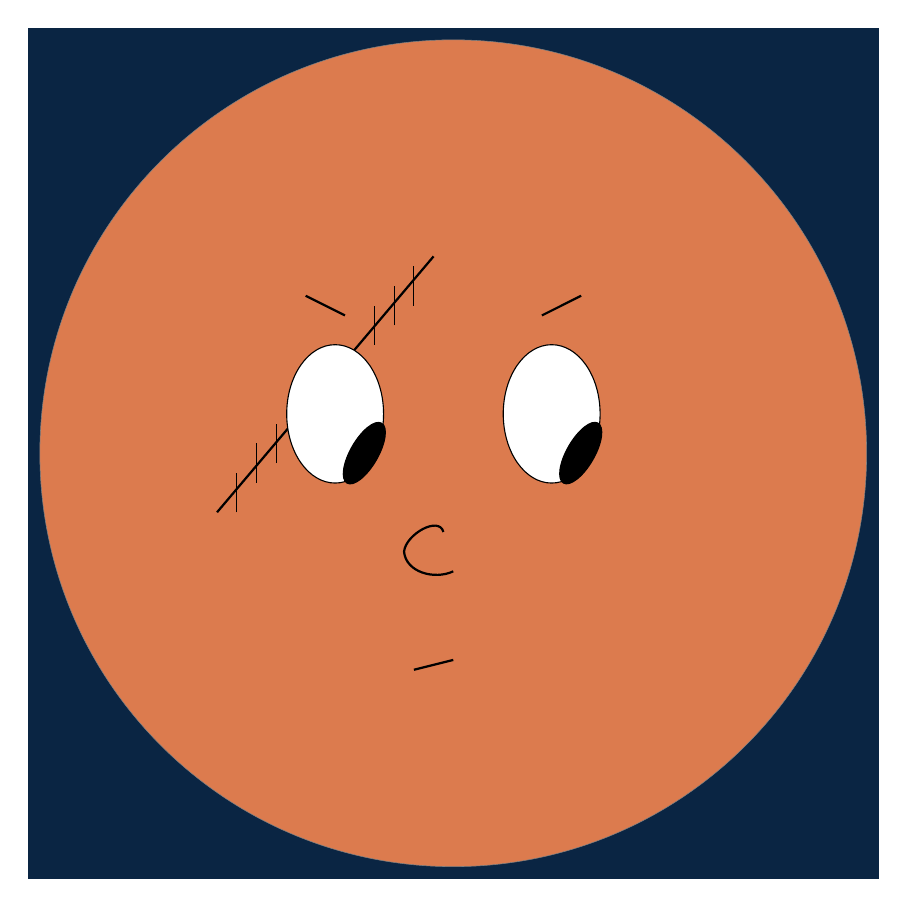
\begin{tikzpicture}[background rectangle/.style={fill=space},show background rectangle,]
		\begin{scope}[scale=2.5]
			\tkzDefPoint(3,0.5){M}
			\tkzDefPoint(5.1,0.5){R}
			\tkzDefPoint(2.4,0.7){E}
			\tkzDefPoint(3.5,0.7){F}
			%
			\tkzDefShiftPoint[E](0.15,-0.2){E1}
			\tkzDefShiftPoint[E](-0.15,-0.2){E2} %for pupils at left
			\tkzDefShiftPoint[F](0.15,-0.2){F1}
			\tkzDefShiftPoint[F](-0.15,-0.2){F2} %for pupils at left
			%
			\tkzDrawCircle[fill = mars](M,R)
			%scar
			\draw[-,thick] (1.8,0.2) -- (2.9,1.5);
			\draw[-] (1.9,0.2) -- (1.9,0.4);
			\draw[-] (2,0.35) -- (2,0.55);
			\draw[-] (2.1,0.45) -- (2.1,0.65);
			\draw[-] (2.6,1.05) -- (2.6,1.25);
			\draw[-] (2.7,1.15) -- (2.7,1.35);
			\draw[-] (2.8,1.25) -- (2.8,1.45);
			%eyebrows
			\draw[-,thick] (2.25,1.3) -- (2.45,1.2);
			\draw[-,thick] (3.45,1.2) -- (3.65,1.3);
			%nose
			\draw[-,thick] (2.95,0.1) to[out=105,in=85] (2.75,0) to[out=275,in=205] (3,-0.1);
			%mouth
			\draw[-,thick] (2.8,-0.6) -- (3,-0.55);
			%eyes
			\draw[fill=white] (E) ellipse (7pt and 10pt);
			\draw[fill=white] (F) ellipse (7pt and 10pt);
			%pupils right
			\draw[fill=black,rotate around={-30:(E)}] (E1) ellipse (2pt and 5pt);
			\draw[fill=black,rotate around={-30:(F)}] (F1) ellipse (2pt and 5pt);
			%pupils left
			%\draw[fill=black,rotate around={30:(E)}] (E2) ellipse (2pt and 5pt);
			%\draw[fill=black,rotate around={30:(F)}] (F2) ellipse (2pt and 5pt);
		\end{scope}
	\end{tikzpicture}
\end{document}